% Preamble
\documentclass[11pt]{article}

% Packages
\usepackage{amsmath}
\usepackage{float}
\usepackage[T1]{fontenc}
\usepackage{lmodern}
\usepackage[polish]{babel}
\usepackage[utf8]{inputenc}
\usepackage{polski}
\usepackage{hyperref}
\usepackage{graphicx}
\setlength{\parindent}{0pt}

% Document
\begin{document}

    \title{Projekt SPIN nr 2 - CorpoFiszki}
    \author{Bartosz Walusiak, Rafał Łyżwa}
    \date{\today}
    \maketitle

    \tableofcontents

    \newpage

    \section{Opis projektu}\label{sec:description}
    \subsection{Cel}\label{subsec:target}
    Cel projektu:\\
    Wykorzystanie środowiska processing do stworzenia prototypu aplikacji pomagającej w nauce imion współpracowników.

    \subsection{Założenia przyjęte w trakcie realizacji}\label{subsec:design-choices}
    Założenia:
    \begin{itemize}
        \item Obsługa aplikacji za pomocą myszki.
        \item Import danych użytkownika za pomocą pliku .csv.
    \end{itemize}

    \subsection{Analiza literatury}\label{subsec:research}

    Do realizacji projektu wykorzystaliśmy przykładowe projekty dostępne na \href{https://processing.org/examples/}{stronie processingu}.
    \begin{enumerate}
        \item Wczytywanie danych z \href{https://processing.org/examples/loadsavetable.html}{tabeli}.
        \item Wczytywanie i wyświetlanie \href{https://processing.org/examples/loaddisplayimage.html}{obrazków}
    \end{enumerate}

    \subsection{Prototyp}\label{subsec:prototype}

    \begin{figure}\label{ss1}
        \centering
        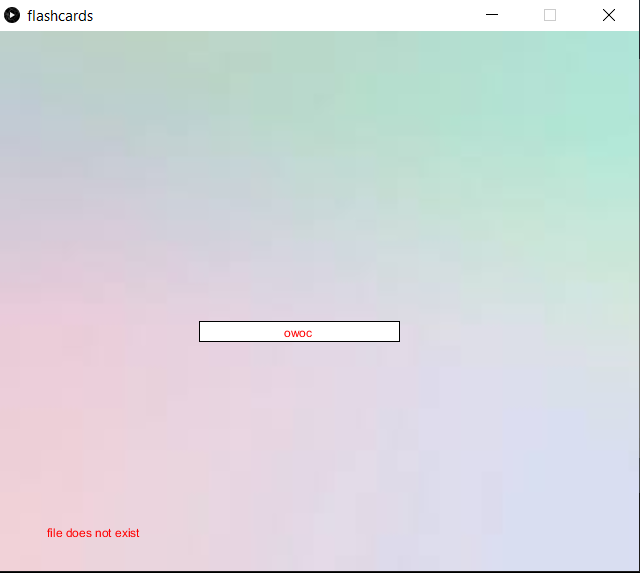
\includegraphics{Screenshot_1.png}
        \caption{Infornacja o błędnym folderze}
    \end{figure}

    \begin{figure}\label{ss2}
    \centering
    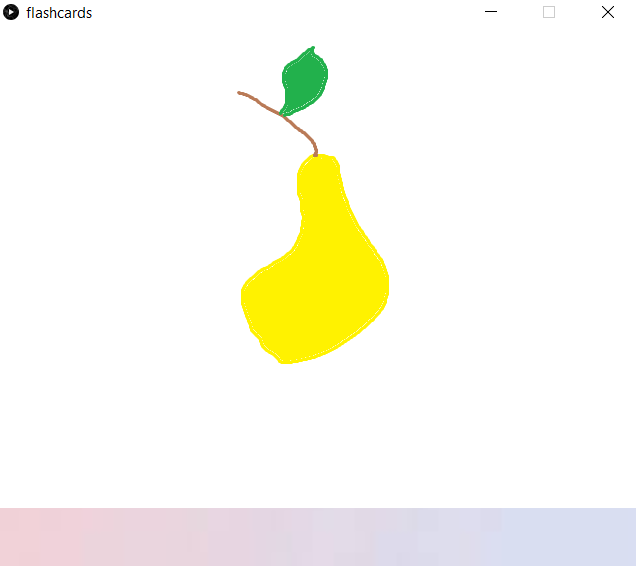
\includegraphics{Screenshot_2.png}
    \caption{Losowy obrazek}
    \end{figure}

    \begin{figure}\label{ss3}
    \centering
    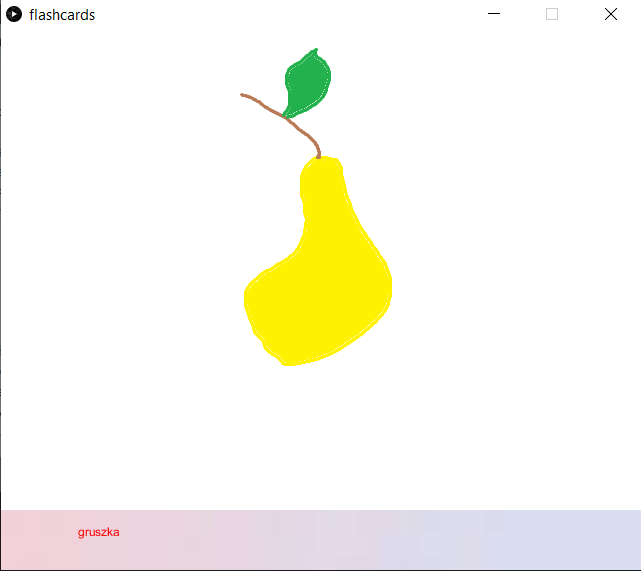
\includegraphics{Screenshot_3.png}
    \caption{Nazwa przypisana do obrazka}
    \end{figure}

    \newpage

    \section{Instrukcja obsługi}\label{sec:user-manual}

    \subsection{Uruchomienie aplikacji}\label{subsec:setup}

    \begin{enumerate}
        \item \href{https://github.com/BWalusiak/flashcards/releases}{Pobierz} najnowszą wersję aplikacji dla odpowiedniego systemu z repozytorium.
        \item Odpakuj do wybranego folderu.
        \item Uruchom.
    \end{enumerate}

    \subsection{Import danych}\label{subsec:data-import}

    \begin{enumerate}
        \item Przy uruchomieniu aplikacji podaj folder z danymi.
        \item Potwierdź klawiszem enter.
    \end{enumerate}


\end{document}